\documentclass[12pt]{article}
\usepackage{array}
\usepackage{graphicx} % Allows including images
\usepackage{booktabs}
\usepackage{tabularx}
\usepackage{siunitx}
\usepackage{ragged2e} 
\usepackage{amssymb,amsmath,amsfonts,booktabs,eurosym,geometry,ulem,graphicx,caption,color,setspace,sectsty,comment,footmisc,caption,natbib,pdflscape,subfigure,array,hyperref, tabularx, siunitx, ragged2e}
\usepackage{float}
\usepackage{subcaption}

\normalem

\onehalfspacing
\newtheorem{theorem}{Theorem}
\newtheorem{corollary}[theorem]{Corollary}
\newtheorem{proposition}{Proposition}
\newenvironment{proof}[1][Proof]{\noindent\textbf{#1.} }{\ \rule{0.5em}{0.5em}}

\newtheorem{hyp}{Hypothesis}
\newtheorem{subhyp}{Hypothesis}[hyp]
\renewcommand{\thesubhyp}{\thehyp\alph{subhyp}}

\newcommand{\red}[1]{{\color{red} #1}}
\newcommand{\blue}[1]{{\color{blue} #1}}

\newcolumntype{L}[1]{>{\raggedright\let\newline\\arraybackslash\hspace{0pt}}m{#1}}
\newcolumntype{C}[1]{>{\centering\let\newline\\arraybackslash\hspace{0pt}}m{#1}}
\newcolumntype{R}[1]{>{\raggedleft\let\newline\\arraybackslash\hspace{0pt}}m{#1}}

\geometry{left=1.0in,right=1.0in,top=1.0in,bottom=1.0in}

\begin{document}
\title{Divergence of Collective Memory on European Financial Entrenchment -
Implications for the European Union (working title)}
\author{Laura Arnemann, Kai A. Konrad and Niklas Potrafke}
\maketitle

\begin{abstract}
We examine the extent to which collective memory on the 2010 European debt crisis differs between citizens from borrower and lender countries. We employ new survey data for economic experts and non-experts. The results do not suggest that experts from borrower countries have different views than experts from lender countries. Economic expertise may well help to remember issues of the European debt crisis and to prevent nation-serving bias. By contrast, non-experts from borrower countries have different memories about the crisis than non-experts from lender countries. There is evidence for a nation-serving bias. Our results suggest that public debt relationships between nations influence how citizens of the individual countries perceive the contracting countries.
\end{abstract}
\clearpage
\section{Introduction}

We examine collective memories of the European debt crisis that
began in 2010: memories of experts and non-experts, considering whether they are from program countries or non-program countries.
The European debt crisis partitioned the countries inside the Eurozone. Some
Eurozone member countries experienced fiscal and financial conditions that
dramatically worsened and were in danger of losing access to the capital
market for refinancing their public loans. The other countries had to
fear contagion effects and spillovers of possible national
bankruptcies in the more severely affected countries.\ Five countries
(Greece, Ireland, Portugal, Spain and Cyprus) applied for, and signed a
memorandum of understanding with the member countries of the European
Monetary Union. They received financial aid or
guarantees and accepted supervised mandatory structural reforms. We refer to the program
countries as the 'borrower countries'. Other countries used their fiscal credibility to provide these guaranties and requested
and participated in a monitoring of the process of structural reforms. We
refer to them as 'lender countries'.

Will citizens from borrower and lender countries have similar memories about who
applied for a memorandum of understanding? How do they remember
whether the lender or the borrower countries pushed for the memoranda of understanding and whether
the memoranda of understanding mainly benefited the lender countries or the
borrower countries? And if there are differences between borrower and lender countries, do these differ between economic experts and non-experts? We also
investigate how the programs were perceived in the countries
and how the crisis interventions influenced the relationship between
countries.\ 

We consider the views of experts polled by CESifo's World Economic Survey (WES) panel of experts and non-experts in European countries in an internet questionnaire (https://prolific.co) to answer the same questions. The results do not suggest that the answers between experts from borrower countries and experts from lender countries diverge. However, differences emerge in how non-experts from the borrower and lender countries remember which countries signed a memorandum, why they signed it, and how they assess the measures taken to address the crisis. We employ data from 2018/2019 (experts/non-experts) and examine whether the borrower or lender position predicts how the crisis is remembered and assessed. 

Memory formation has been primarily studied in psychology, neuroscience and sociology.
Insights about the plasticity of memory\footnote{%
The physiological basics for how memory is formed, kept and reactivated have
been explored. As Dudai and Edelson (2016;\ 276)\ describe, "When the memory
is retrieved, it seems to re-enter a transient phase in which it again
becomes susceptible to the same amnesic agents that were effective in the
original consolidation window (\cite{dudai}; \cite{nader}; Sara,
2000)." Brain sciences hence suggest that memory enters a state of
plasticity when it is reactivated and the copy that is then stored might
differ from the one that has been activated (see \cite{agren}, and \cite{lee}).}, and a tendency to memorize in a 'self-serving' way
(\cite{bell}) have been combined. If this self-serving bias
affects the process of reactivating, transforming and storing memory, it may well
cause memory with a self-serving bias.

A self-serving bias has been shown in memories of informal credit relationships (\cite{dezso}). Using data about informal credit
relationships between relatives and friends, \cite{dezso} find that borrowers and
lenders diverge in their memories about these credit relationships in self-serving
 ways.
Borrowers and lenders remember in different manners the credit event
as such, the conditions of the loan they agreed upon, and the mutual
interactions that made the contract come about. This divergence typically
has a self-serving bias. For instance, compared to the lenders, borrowers
tend to recall less if they exerted moral pressure to receive the loan and
are more likely to recall that the credit was generously offered to them.

The lenders and borrowers in the European debt crisis are
nations, no individuals, but the line of reasoning may well be
similar: when investigating the recollections of fiscal credit relationships or
loan guarantees between nations, the mental processes of the formation,
storage and reactivation of memory are still those of individuals.
The formation of memories of individuals who belong to the same group might
follow the same logic and physiological laws as in private
borrowing-lending relationships. Overall, individuals in borrower
countries and individuals in lender countries might recall differently
aspects of the credit relationship similar to individuals in a private credit relationship. 

\\

Diverging views and memories might be reinforced 
by biased public news and newspaper reports. Common
institutions inside a nation, such as common exposure to the same public
media and other public institutions might intensify information exchange
inside the group, might cause a continuous transformation of this aggregate
and might even strengthen and homogenize the national collections of
memories. For discussions see \cite{rigney} and Roediger and Abel (2015;\
361) who conclude: "Such collective memories probably boost group identity
and shape social and political discourse. In particular, studies of how
various groups remember `the same' events so differently may help to uncover
important psychological factors in group dynamics and conflict." \cite{baumeister} describe that groups employ techniques such as selective omission, fabrication of alternative narratives and exaggeration or embellishments of events to let their group appear in a favorable light. \cite{abel} show self-serving group bias in country's assessment of the Second World War. Citizens overestimate their country's contribution to the Second World War. 

We relate to studies which investigate how views of economic experts and non-experts differ. \cite{johnston} find that citizens are influenced by the views of economic experts, more so if the issue at stake is highly technical and less ideological. However, the issue at stake does not appear to be the only determinant of divergence in the views of experts and non-experts. In a survey of economic experts and a representative sample of the U.S. population \cite{sapienza} find that NIKLAS: WAS BEDEUTET DER KOMMENDE HALBSATZ? the divergences in opinions is increasing in the level of agreement among economic experts. The WES has also been employed to measure discrepancies in the views of experts and non-experts. \cite{roth} find that experts and non-experts assess the impact of macroeconomic shocks differently.

Our study is also related to studies in political science.
%We conduct an inter-country comparison  of memories of the events surrounding the European debt crisis and compare the memories of economic experts to regular citizens. 
\cite{bechtel} examine how the political orientation of German citizens influences attitudes towards the European debt crisis. The results show that traditional left/right cleavages do not explain participants perception of the European debt crisis but rather moderateness of political views. More cosmopolitan survey participants are less opposed to the European rescue program. This finding is corroborated by \cite{kuhn} who use survey data: ``cosmopolitans" have a lower propensity to discriminate between national recipients of transfers and international recipients of transfers than non-cosmopolitans. We designed a survey specific to the European debt crisis and ask experts and non-experts in European Union member states. We compare the memories of economic experts and non-experts. Examining a nation-serving bias in memorizing the European debt crisis is new. 



\section{Related Literature}

\section{The surveys }
Our data was obtained through surveys that were conducted among two pools of
participants. In August 2018, we asked economic experts from the World
Economic Survey (WES) for their opinion on perceptions about the financial
entrenchment following the European debt crisis. The WES is a quarterly
survey conducted by the ifo Institute. The WES sample includes 517
participants from EU member countries, among them 90 experts from program countries.
The survey regularly includes questions about overall economic development
from European and non-European experts such as economic growth and
inflation. The WES in August 2018 included a special module with a set of
questions on the European debt crisis (see the Appendix for the
questionnaire). \footnote{Scholars use the WES to include special modules. See, for example, \cite{mosler}.}

Our second pool of participants was recruited through the website
prolific.co. In contrast to other crowdsourcing platforms such as Mturk,
Prolific is a platform specifically designed to recruit participants for
academic research \footnote{\cite{Peer} demonstrate that participants from
the platform prolific perform better than participants from other
crowdsourcing platforms.}. In exchange for their participation in surveys or
experiments, participants receive a financial reward. The survey was
distributed to 1702 participants in August 2019, 498 of these participants
came from program countries. To ensure that our participants had an
opportunity to actively remember the events during the European debt crisis
we restrict our sample to include only participants older than 25.

The precisely same survey questions were used in both surveys, and in
unchanged ordering. The appendix shows the country composition of survey
participants for both samples.\footnote{%
The WES sample and the prolific sample naturally differ along various
dimensions. The differences are largely due to the expert status of members
of the WES sample. The majority of participants from the prolific sample,
around 65 percent are younger than 35, whereas the majority of participants
from the WES sample are between 35 and 55. Participants from the WES sample
are also have a higher level of education than participants from the
prolific sample, 60 percent of participants hold a PhD. Nonetheless the
majority of participants from the prolific sample have completed tertiary
education. More than 80 percent of WES participants are male, whereas in the
prolific sample there is an equal share of men and women.} We refer to the
WES sample as the expert sample and to the prolific sample as the non-expert
sample. We are interested in whether the survey participants show a
nation-serving bias in their answers, and whether there is a structural
difference between replies by ordinary citizens and by experts.

\section{Questions, hypotheses and findings}

The questionnaire starts with recalling the European debt
crisis that began in 2010, and the memoranda of understanding
that Greece, Spain, Portugal, Ireland and Cyprus signed with the European
Union, the European Central Bank and the International Monetary Fund that  
established financial aid combined with economic adjustment. We refer to
these contracts as \textit{aid\&reform} programs. 
We investigate whether country
origin matters for respondents' opinions about the reasons for why lender countries wanted to engage in the credit relationship. 
\begin{figure}[h!]
\caption{Reasons of the lender countries for entering the rescue program}
    \begin{center}
    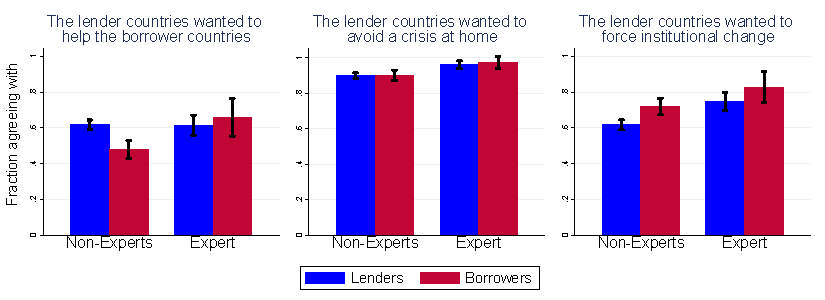
\includegraphics[scale=1.2]{graph2.pdf}
    \label{fig:Figure1}
    \end{center}
     \tiny
     \begin{tablenotes} 
    {The exact wording of the question is: In your opinion, what is the main reason why these countries entered these programmes 2a The lender countries wanted to help the borrower countries; 2b The lender countries wanted to help themselves to avoid a major crisis at home; 2c The lender countries wanted to force their desire for institutional change upon the borrower countries. Participants could choose the options strongly agree, slightly agree, slightly disagree and I don't know. We exclude all participants who answered with I don't know.\\
    The whiskers represent the 95 \% confidence intervals}
    \end{tablenotes}
\end{figure}

The nation-serving hypothesis is:\ respondents from borrower countries tend
to agree less frequently than respondents from lender countries 
that the lender countries wanted to help. They agree more that
the lender countries wanted to help themselves, and they agree more 
often that the lender countries wanted to force institutional change on the
crisis countries.\textit{\ }

The nation-serving hypothesis is not rejected based on our data (\autoref{fig:Figure1}). The share of non-experts from lender countries agreeing that lender countries wanted to help the borrower countries (62\%) is larger than the share of non-experts from borrower countries (48\%).
The difference in assessments between
non-experts from borrower and lender countries are large and statistically
significant at the 1 \% level for this aspect of the reforms. There is also some disagreement in the expert sample. The differences, however, do not turn out to be statistically significant. \\
It is conceivable that
many non-expert respondents in the borrower countries believe that
the lender countries had an institutional-reform agenda that goes beyond the
idea of helping each other. Participants from borrower and lender countries agree that lender countries wanted to avoid a crisis at home both in the expert and non-expert sample. The nation-serving bias manifests itself again in the non-expert sample in the question about the desire for institutional change among the lender countries. 62 \% of non-experts from lender countries agree with this statement compared to 72 \% among the lender countries. Again, we observe differences in answers among the expert sample as well which do not turn out to be statistically significant. 
It is conceivable that experts, apart from simply being
better informed, often identify less with their own countries of origin and have 
a more cosmopolitan orientation. Therefore, the
forces for developing a nation-bias might be less strong for experts than for non-experts. 

\begin{figure}
    \begin{center}
      \caption{Driving Force and Beneficiaries}
    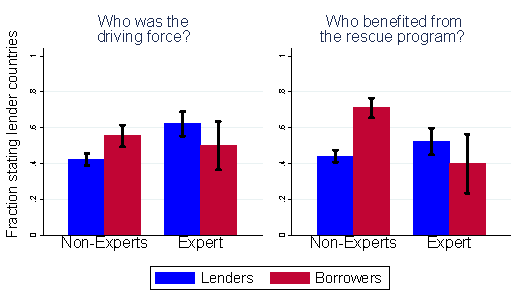
\includegraphics[scale=1.2]{graph3.pdf}
  
    \label{fig:figure2}
    \end{center}
    \tiny
    \begin{tablenotes} 
    {The exact wording of the questions is: 3. In formal terms, the borrower countries that signed a memorandum had to apply for support. But thinking about the true motivations and the political processes behind these events, which of the following three alternatives corresponds most closely to your perceptions. Answer options: The borrower countries wanted it, the lender countries were more reluctant; The lender countries wanted it, the borrower countries were more reluctant; Both wanted it equally; I don't know \\
   Question 4: Who do you think mainly benefited from the rescue program. Answer options: The borrower countries; The lender countries; Both groups of countries benefited equally; I don't know. We exclude all participants who answered with I don't know. \\
   The whiskers represent the 95 \% confidence intervals.}  
    \end{tablenotes}
\end{figure}
The following questions corroborate that the difference in nation-serving bias is a more systematic pattern (\autoref{fig:Figure1}). They show very similar patterns for non-expert
respondents, depending on whether they are from borrower countries or from
lender countries. The results suggest large and significant nation-biases. Question 3 is similar to Question 2 and asks the respondents about the driving force behind the \textit{aid\&reform programs}. Question 4 asks about the main beneficiaries of the aid&reform program. Non-experts
from borrower countries tend to see the lender countries as the main
motivators for these programs. This result corroborates the results on
self-serving memories from private informal lending as in \cite{dezso}, who report a tendency to assign the initiative\
for such contracts to the other side of the credit relationship. 

Non-experts from borrower and lending countries also differ in
their perceptions of who mainly benefited from the \textit{aid\&reform programs}. The
bias tends to assign the benefits more to the counterparty group:\
respondents from borrower countries think more often than respondents from
lender countries that the lender countries are the major beneficiaries. 

The responses of experts do not seem to be prone to a country-group
bias. Whether an expert is originally from a borrower country or a lender
country does not affect their assessments about the
motivations driving the \textit{aid\&reform programs}, nor their assessments about
who was the main beneficiary.\footnote{98 percent of experts also works in their country of origin }  Interestingly, there is a nation-disfavoring bias in the sample of experts. Experts from lender countries are 12 percentage points more likely to agree that lender countries were the driving force and the main beneficiaries of the rescue program (\autoref{fig:figure2}). However, these differences do not turn out to be statistically significant.

We now turn to questions addressing how the groups of respondents
assess the implications of the \textit{aid\&reform programs} for feelings among the
populations in the borrower and the lender
countries. The respondents' perceptions might be formed by direct
observations in the countries or media reports, but their views about the
reasons and motivations for the \textit{aid\&reform programs} and their views about
who actually benefited from these programs should correlate with their
assessments, and might cause their beliefs about these feelings. 

We ask whether respondents think that the rescue experience might
have caused feelings of \textit{guilt}, feelings of \textit{being
exploited}, and/or feelings of \textit{inferiority}. These questions do not directly reflect a nation-serving bias but might rather be the outcome of such a bias. For example, a respondent from Greece might think that the \textit{aid\&reform programs} mainly benefited the lender countries which forced Greece to undertake the reforms. Hence, a Greek respondent might not feel guilty due to the \textit{aid\&reform programs}. On the other hand, a respondent from the lender countries might feel that the \textit{aid\&reform programs} was a benevolent gesture from the lender countries which provided large benefits to the program countries. Hence, a respondent from the lender countries might be more prone to assume that citizens in the borrower countries felt guilt due to the large benefits they received.\footnote{Our findings can also be interpreted in an alternative way.  Having a self-serving or nation-serving bias might make individuals oblivious to
the way policies are received in other countries. 
\cite{dezso} refer to this phenomenon as having a ``blind spot" regarding the other party's 
feelings and emotions. The hypothesis on the existence of such a ``blind spot" is confirmed in our findings.
Citizens from lender countries are more likely to agree that they felt guilty, exploited and/or inferior as a 
consequence of the \textit{aid\&reform programs}. The largest difference between lender and borrower countries occurs with regards to feeling exploited.
78 percent  of citizens from borrower countries state that they felt exploited due to the \textit{aid\&reform programs} while only 61 percent of lender countries
agree to this statement. 
}

%Similar reasons might let us suspect that the respondents from the lender
%countries are more inclined to think their population feels exploited, or
%feel inferior (in the sense of humiliated). Figure xxx shows the answers.
%First statistics negate the existence of a blind spot among borrowers about the feelings
%from citizens to lender countries. 

\begin{figure}
\begin{center}
    \caption{Emotions of the borrower countries}
    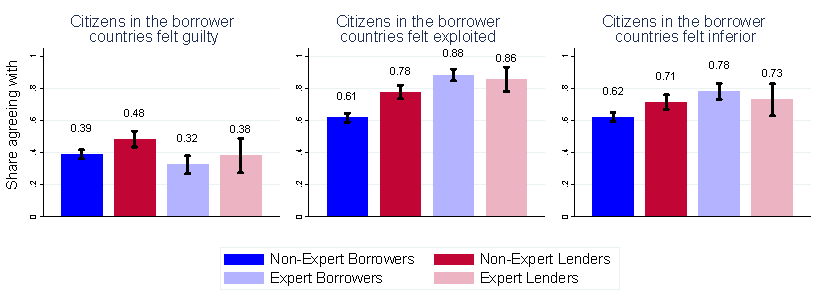
\includegraphics[scale=1.2]{graph5_1.pdf}
    \label{fig:figure3}
    \end{center}
    \tiny 
      \begin{tablenotes} 
      {The exact wording of the question was the following: Please give assessments of the following questions: 5a) The rescue experience made many citizens in the borrower countries feel guilty 
      5b) The rescue experience made many citizens in the borrower countries feel exploited 5c) The rescue experience mad many citizens in the borrower countries feel inferior
      Answer options: strongly agree, slightly agree, slightly disagree, strongly disagree, I don't know. We exclude all participants who answered with I don't know. \\
      The whiskers represent the 95 \% confidence intervals.}
      \end{tablenotes}
\end{figure}

As expected the view of experts is not influenced by their countries of origin.  (\autoref{fig:figure3}).


Similar questions assess the perceptions in the groups about the
feelings in the lender countries. In particular, we asked the participants whether they
agree that the \textit{aid\&reform programs} made the citizens in the
lender countries feel exploited and disappointed (\autoref{fig:figure4}). Differences in the answers to these questions might manifest themselves as a consequence of  a nation-serving bias. If citizens from lender countries feel that the borrower countries were the driving force behind the \textit{aid\&reform programs} and also the party which reaped the highest benefit from these programs, they might report to feel exploited. If borrower countries feel they did not benefit from the program and also did not initiate the program, they will infer that lender countries should have no reason to feel guilty. Overall, we might expect that the lender-country respondents agree more
frequently than the borrower-country respondents to the possibly negative
feelings in lender countries.

\begin{figure}[h!]
  \begin{center}
       \caption{Emotions of the lender countries}
    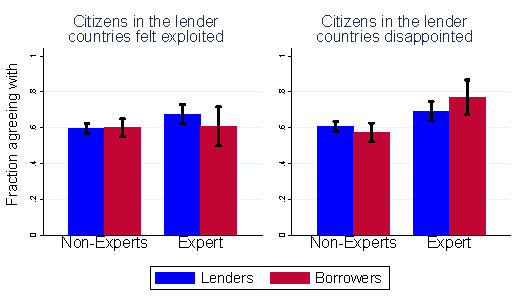
\includegraphics[scale=1.2]{graph5_2.pdf}
 
    \label{fig:figure4}
    \end{center}
    \tiny
    \begin{tablenotes}
     {The exact wording of the question is: 5d) The rescue experience made many citizens in the lender countries feel exploited 5e) The rescue experience made many citizens in the lender countries feel disappointed
    Answer options: strongly agree, slightly agree, slightly disagree, strongly disagree, I don't know. We exclude all participants who answered with I don't know. \\
    The whiskers represent the 95 \% confidence intervals}
    \end{tablenotes}
\end{figure}

The results do not suggest that respondents from borrower countries have different views than respondents from lender countries. The findings indicate that the respondents
in both groups of countries believe that the \textit{aid\&reform programs} triggered
negative feelings in both groups of countries. A large share of the respondents
thinks that citizens in borrower countries feel guilty, exploited, and
inferior, and a large share of respondents also thinks that citizens in
lender countries feel disappointed and exploited as well. 

We also ask whether the \textit{aid\&reform programs} strengthened friendship between the citizens in the Eurozone. The theory of groups and conflicts shows that, when groups jointly master a major task which none of them could have mastered alone, they overcome negative attitudes and mutual spite between groups HABEN WIR HIERZU REFERENZEN ZUM ZITIEREN?. The European debt crisis had the potential to be 
such a task. It might have strengthened friendship between these groups.
However, if both groups have nation-serving biases about what
motivated the crisis and the solution method adopted, and about the
distribution of the benefits and costs of the method adopted, then we might
expect that a large fraction of the respondents of both groups think that
these programs did not strengthen friendship ties. 
\begin{figure}
\begin{center}
\caption{Impact on friendships}
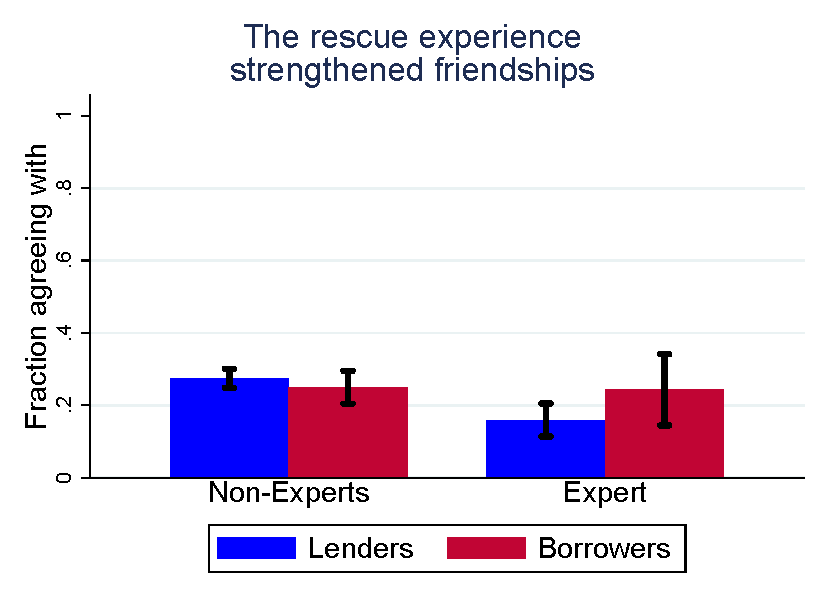
\includegraphics[scale=0.5]{graph5_3.pdf}
\label{fig:figure5}
\end{center}
\tiny 
\begin{tablenotes}
  {The exact wording of the question is the following: 5f) The rescue experience strengthened friendships
   Answer options: strongly agree, slightly agree, slightly disagree, strongly disagree, I don't know. We exclude all participants who answered with I don't know. \\
     The whiskers represent the 95 \% confidence intervals}
    \end{tablenotes}
\end{figure}

The majority of participants from the expert and non-expert sample disagrees that 
the rescue package strengthened friendships (\autoref{fig:figure5}).\footnote{Due to a survey error this question was displayed as "The rescue experience strengthened friendship ties between borrower". The fraction of experts who answered this question with "I don't know" lies around 20 percent. This is very much in line with the frequency of "I don't know" responses throughout the survey. Hence, it seems plausible that participants correctly understood the question. } This holds for participants from 
both the expert and the non-expert sample. This finding suggests that non-experts are aware of the divergence of views between lender and borrower countries and tensions arising from such divergences. In light of the absence of such a bias among the expert sample 
it seems interesting that the level of agreement in this sample is also quite low. 
This might suggest that although experts might not have and be aware of a nation-serving bias
among citizens from the lender countries they are indeed aware of the consequences of such 
a nation-serving bias. 



\clearpage
\section{Results}
We present the results of our empirical analysis for the sample of experts (the WES sample) and the sample of non-experts (the prolific sample).  We estimate the following model using binary logit. 
\begin{equation*}
    Y_{ijc}= \alpha_{j}+ \beta *D_{c} + \gamma*X_{i}
\end{equation*}
Where $Y_{ijc}$ denotes the response of individual $i$ from country $c$ to question $j$ we will control for individual characteristics $X_{i}$ such as age, level of education, gender and employment status (affiliation for the expert sample). The dummy variable $D_{c}$ indicates whether the expert's nationality is Greek, Cypriotic, Spanish, Irish or Portuguese with the coefficient $\beta$ measuring the divergence in the answers of participants from program and non-program countries. \footnote{In the expert sample participants are asked in which country they were born}For questions in which participants were asked to state their level of agreement we estimate the effect of being from a program country on the likelihood to strongly or slightly agree. For questions in which participants are asked to name the responsible party, we estimate the effect of being from a program country on the likelihood to state "Lender countries". \\ \\
\textbf{Baseline Results} 
When asked about the intentions of lender countries to initiate the credit relationship our hypothesis is verified among our non-expert participants.
 In the non-expert sample citizens from program countries are 10.9 percentage points more likely to agree that lender countries wanted to impose institutional change upon the borrower countries. They are 13.1 percentage points less likely to agree that the lender countries wanted to help the borrowing countries. However, there is no significant effect on agreeing that lender countries merely wanted to avoid a crisis at home. In the expert sample there are no statistically significant differences in the assessments of experts from program and non-program countries. Contrasting our hypothesis,  experts from program countries are more likely to agree that the lender countries wanted to help the borrowing countries. This effect does not turn out to be statistically significant.  \\ 
 \begin{figure}[H]
\begin{center}
     \caption{ Hypothesis 1: Why the lender countries initiated the credit relationship}
    
     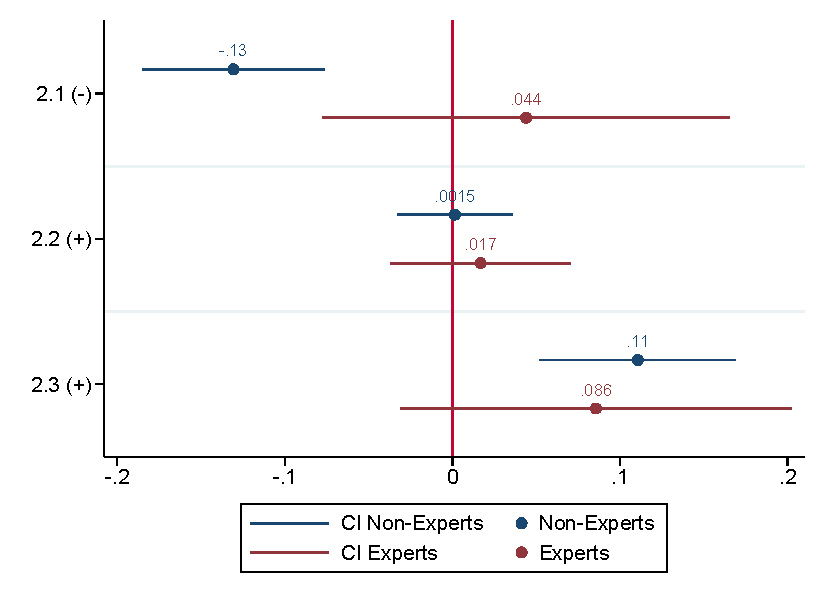
\includegraphics[scale=0.8]{Question2_base.pdf}
     \label{fig:my_label}
      \end{center}
      \tiny
     \tablenotes{The sign in parantheses denotes the predicted differential effect. Participants were asked to assess the following statements:  Question 2.1: The lender countries wanted to help the borrowing countries Question 2.2: The lender countries wanted to help themselves avoid a crisis at home Question 2.3: The lender countries wanted to impose institutional change upon the borrower countries  }
\end{figure}
 We continue to ask the participants about the emotions the rescue program evoked among citizens from the borrower and lender countries. The hypothesis that lenders have a blind spot regarding the feelings of citizens from borrower countries is confirmed. Participants from program countries in the non-expert sample are 9.2 and 9.3 percentage points more likely to agree that the rescue experience made them feel guilty and inferior. Further, the probability to agree to "The rescue experience made many citizens in the borrower countries feel exploited" increases by 16.9 percentage points among citizens from program countries. All effects are statistically significant at the 1 percent level. Among the sample of economic experts the effect sizes are smaller and not significantly different from zero. \\
 Interestingly, we do not find that borrowers have a blind spot regarding the emotions the program evoked among lender countries. There are only small differences in the likelihood to agree with certain statements between citizens from program and non-program countries which are not significant. There is no difference in evaluating the effect of the rescue program on the friendship between citizens. The results are similar in the expert and non-expert sample. \\

 We further predicted that borrower countries will be more confident that they will be able to repay outstanding debt. 
 When asked whether Greece \footnote{We only ask about Greece, since Greece remains the only country that has not repaid it's debt} will be capable of fully paying back it's debt, citizens from program countries show a 13.5 percentage point higher likelihood to agree in the non-expert sample and a 12.2 percentage point higher likelihood in the expert sample. This effect is again significant at the 1 percent level. \\
 \begin{figure} [h!]
    \begin{center}
    \caption{Hypothesis 4: Feelings evoked among citizens from program countries}
    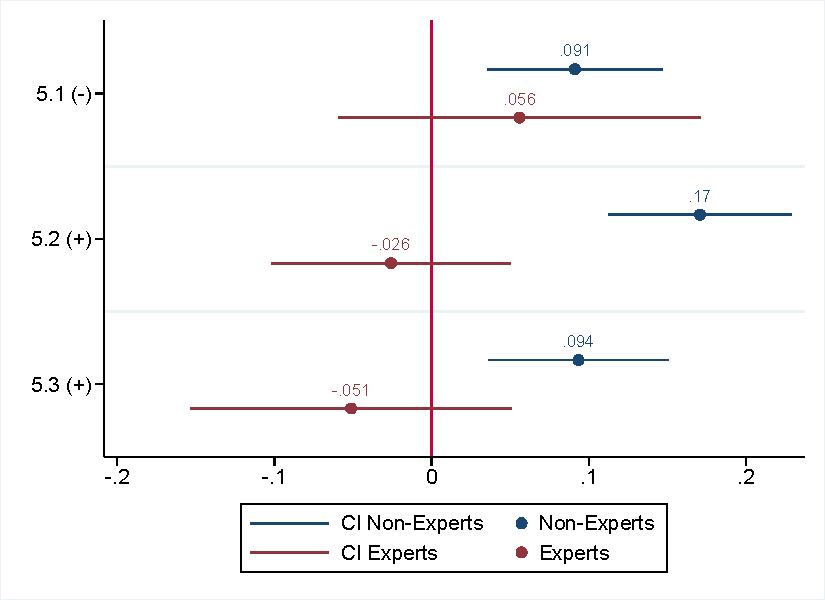
\includegraphics[scale=0.8]{Question5_1_base.pdf}
    \label{fig:my_label}
    \end{center}
    \tiny
    \tablenotes{The sign in parantheses denotes the predicted differential effect. Question 5.1: The rescue experience made many citizens in the borrower countries feel guilty; Question 5.2: The rescue experience made many citizens in the borrower countries feel exploited; Question 5.3: The rescue experience made many citizens in the borrower countries feel inferior. }
\end{figure}
\begin{figure}[h!]
\begin{center}
\caption{Hypothesis 4 and 5: Feelings evoked among citizens from non-program countries }

    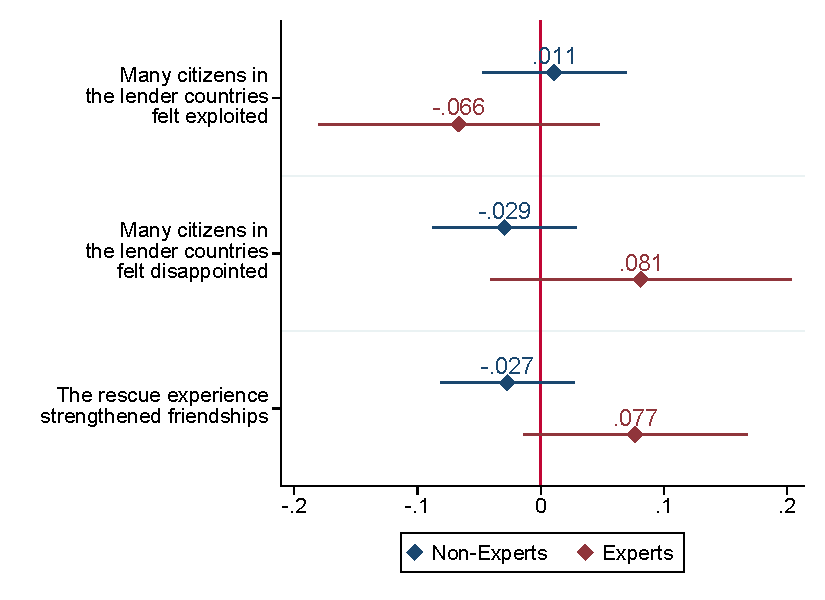
\includegraphics[scale=0.8]{Question5_2_base.pdf}
    \label{fig:my_label}
    \end{center}
    \tiny
    \tablenotes{The sign in parantheses denoted the predicted differential effect. Question 5.4: The rescue experience made many citizens in the lender countries feel exploited; Question 5.5 The rescue experience made many citizens in the lender countries feel disappointed Question 5.6: The rescue experience strengthened friendships between citizens Question 7: Greece will fully pay back it's debt}
\end{figure}
 
%  \begin{figure}
%\caption{Assessment of the emotions the program evoked among different parties}
%\centering
%\begin{minipage}{.5\textwidth}
% 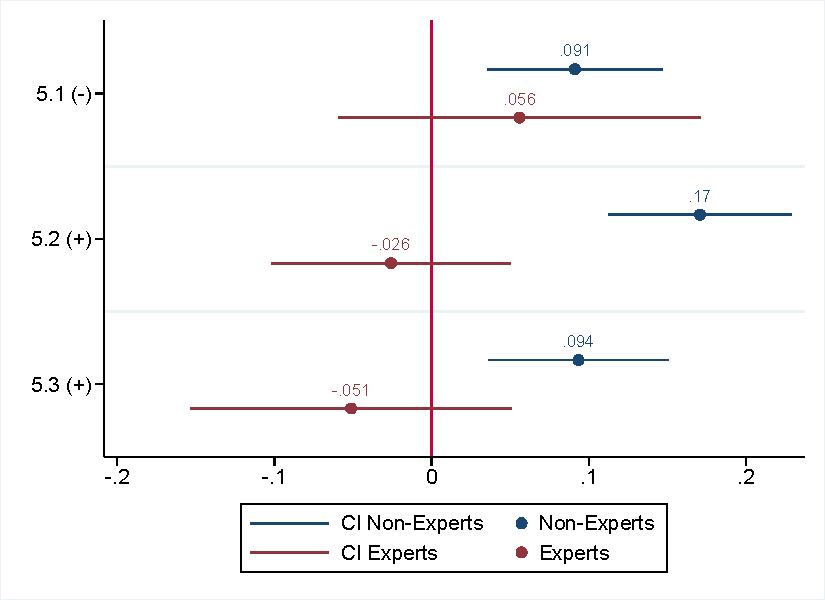
\includegraphics[scale=0.5]{Question5_1_base.pdf}
 %\end{minipage}%
 %\hfill
%\begin{minipage}{.5\textwidth}
%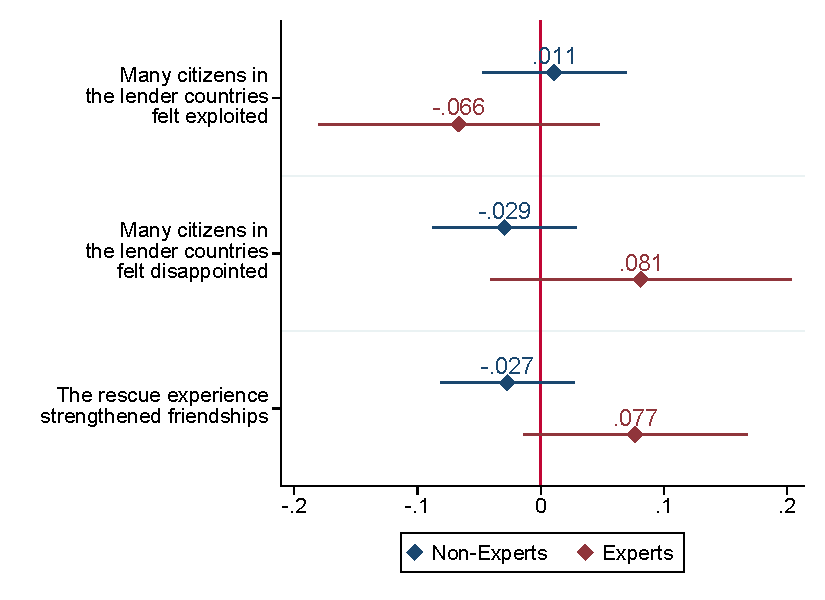
\includegraphics[scale=0.5]{Question5_2_base.pdf}
%\end{minipage}
%\end{figure}
 We proceed to evaluate who initiated and who benefited from the credit relationship. 
In the non-expert sample citizens are 13.2 percentage points more likely to state that the lender countries were the driving force behind signing the memorandum. Further, they are 28 percentage points more likely to state that the lender countries were the main beneficiaries of the program and 20.3 percentage points more likely to state that lender countries benefited from the loans to Greece. All effects are statistically significant at the one percent level. We do not find statistically significant effects in the expert sample. Interestingly, the mean difference between expert and non-experts is negative, contrary to the anticipated effect. Experts from program countries are for example 12.4 percentage points less likely to state that citizens from lender countries were the main beneficiary from the program.\\
\begin{figure}[h!] 
\begin{center}
     \caption{Hypothesis 2 and 3: Who initiated and benefited from the rescue program}
     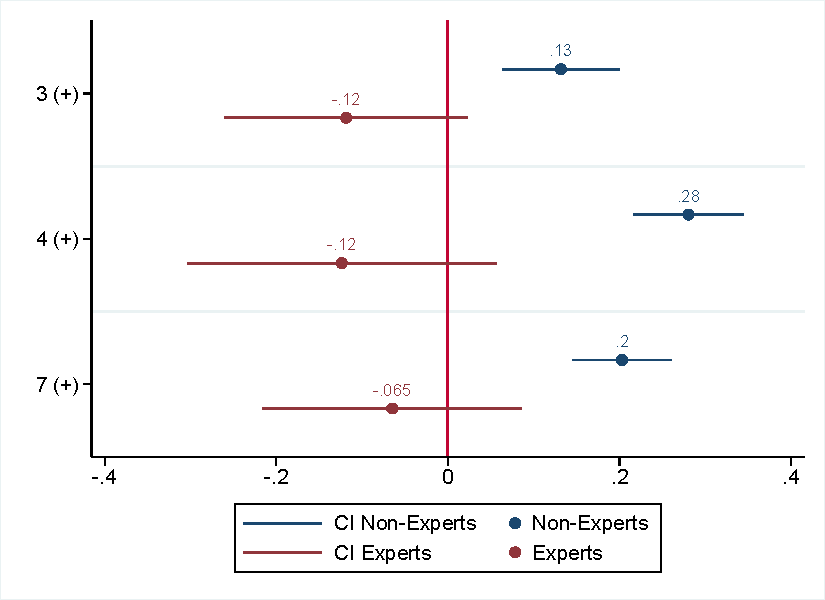
\includegraphics[scale=0.8]{Question3_base.pdf}
     \label{fig:my_label}
     \end{center}
     \tiny
     \tablenotes{The sign in parantheses denotes the predicted differential effect.Question 3: Who was the driving force behind signing the memorandum; Question 4: Who was the main beneficiary of the program; Question 7: Who primarily benefited from the loans to Greece}
\end{figure}

\textbf{Sample Splits}
Program and non-program countries vary along other dimensions than the program and non-program distinction. Program countries have some common characteristics that are likely to influence the estimates. Hence, we conduct sample splits along different macroeconomic variables to assess whether these macroeconomic characteristics influence the magnitude of our effect. Countries which were affected by the European debt crisis are predominantly Southern European and are located at the periphery of the European Union (measured by distance to Brussels). Further, all these countries experienced a substantial increase in debt levels, high levels of unemployment and low GDP growth. We also estimate our model on the subsample of all countries in the Eurozone. In the non-expert sample there are few changes to the baseline results, when splitting the sample along these different characteristics. When asked about the intentions behind entering the rescue program the findings from the baseline regression persist among all sample splits. The effect in the sample of countries with high levels of unemployment becomes smaller and is only significant at the five percent level. In the sample of southern European countries the disagreement over whether lender countries wanted to impose institutional change on borrower countries also decreases and is only significant at the five percent level. Interestingly, the estimates for the sample of periphery countries are much larger than in the baseline sample. In the periphery sample participants from program countries are 19.1 percentage points less likely to agree with the statement that the lender countries wanted to help the borrowing countries and 14.2 percentage points more likely to agree that lender countries wanted to impose institutional change compared to respectively 13.1 and 11.1 percentage points in the full sample.\\
When asked about the emotions of citizens in borrower and lender countries the estimates become slightly smaller in the southern European, periphery and high debt sample than for the full sample. The divergence in assessments about whether the rescue program made the citizens in the borrower countries feel inferior even becomes insignificant in the Southern European sample. Among all samples there is substantial disagreement between program and non-program countries that Greece will repay it's debt. 
\\
The magnitude and significance levels of effects of the program variable remains relatively unchanged for the remainder of questions. There are no differences in the effects of the full sample and all subsamples when asked about the driving force behind the referendum. Further, there is no difference in effects across samples when asked about the main beneficiary of the program. A detailed overview of the results across all sample splits is included in the appendix. 
%\section{Heterogeneity Analysis and Robustness Checks}
Our results show that experts and non-experts show differences in their assessment of the European debt crisis. This finding is in line with work by \cite{roth} who using the WES and a representative sample show that experts differ from non-experts in their beliefs about the impacts of macroeconomic shocks. In our heterogeneity analysis we investigate which difference drives the observed results. We also examine whether individual factors influence the magnitude of the observed divergence. 
\\



\textbf{Socioeconomic Characteristics}
 Experts and non-experts differ along various dimensions such as education, age and gender.
 According to \cite{baumeister} events experienced at a younger age might have a more defining impact. Since the European debt crisis was accompanied for example by a high level of youth unemployment it might seem plausible that the divergences in memory might be more pronounced among the younger generation. Thus, we estimate the effect of belonging to a program country among participants older than 35 among the sample of non-experts.  The effect of the program variable on the likelihood to agree that the lender countries wanted to impose institutional change or that the rescue experience made citizens in the borrower countries feel guilty is smaller and the significance level decreases to 5 percent. For the remaining questions the overall magnitude and significance level of the program effect stays the same. 
\\
The level of education of participants may well influence the estimates. Participants with a higher level of education might have different political attitudes or consume and access different types of media. Hence, we split the non-expert sample and estimate our model only for participants reporting to have completed tertiary education. We do not find any change in the magnitude and significance level of effects for this subsample. 
\\
One dimension along which experts and non-experts differ is their degree of mobility. Experts working in think tanks or research institutes might live or have studied abroad for some time. Due to this circumstance experts might identify less with their nation than non-experts and consequently will not have a strong nation-serving bias. Unfortunately we don't have information about whether participants in the non-expert have lived or studied abroad. However, we can identify if people reported to be living in a different country than their country of birth. This applies to 25 percent of the non-expert subsample. 20.72 percent of participants from program countries and 25.45 percent from non-program countries report to be living in a different country than their country of birth. Estimating our model for this subsample changes the results quite a bit. Divergence between citizens from program- and non-program countries remains in the assessment if lender countries wanted to help borrowing countries and if the rescue experience made the citizens in the borrower countries feel exploited. For the other questions the difference in answers between program- and non-program countries becomes smaller and even vanishes completely for some questions. Hence, it appears that a higher level of mobility might be causal for the differential effects between expert and non-expert sample.  \\

\\
\textbf{Knowledge and beliefs} 
Participants differ in their level of knowledge about the European debt crisis. Some people fail to correctly identify their country as a borrower or lender country. An overview of the fraction of participants who knew their country's status can be found in the appendix. However, knowledge about the status of one's country does not appear to influence the observed effects. The estimates of the baseline model on the subsample of non-experts who could correctly identify their country does not change in comparison to the estimates for the full sample. 

\\\\
We redefine the program variable according to the beliefs of the survey participants. We now estimate the divergence in answers between participants which believed to be the national of a  lender country and participants which believed to be the national of a borrower country. Replacing the program variable by beliefs about belonging to a program country yields different results than the baseline model. In comparison to participants who believe to be lenders, participants who believe to be borrowers do not agree less that lender countries wanted to help borrower countries. They also do not agree more that the rescue program made citizens in the borrower countries feel guilty or inferior and or less likely to state that the lender countries were the driving force behind signing the referendum. Interestingly, differences emerge in the agreement about the feelings of citizens in the lender countries. Participants who believe they live in borrower countries are less likely to agree that citizens in the lender countries felt exploited or disappointed. They are further more likely to believe that the rescue program strengthened friendships between citizens. \\

\\
Our heterogeneity analysis yields some interesting observations about potential drivers of the observed differences between expert and non-expert sample. The comparison of means suggests that the observed differences are not driven by the opinion of experts resembling the opinion of non-experts from either program or non-program countries. 
Our analysis suggests that the observed difference between experts and non-experts cannot be explained by differential effects across age or education levels. However, it appears that non-experts which are more mobile do not show a strong nation-serving bias in their assessments of the European debt crisis. Interestingly, being able to correctly identify one's country as a program or a lender country does not change the observed magnitude of results. The magnitude of effects does change however, when redefining the program variable according to beliefs of people. This suggests that collective memory might work on a more subconscious level regardless of the level of information participants have. 
\\
\\
We also conduct various robustness checks. \\

\textbf{Ordered and Multinomial Estimation}
Participants have multiple answer possibilities. Depending on the question participants are able to rank their level of agreement on a scale of 1 to 4 or choose between the options borrower countries, lender countries or both equally. To control if differences between participants from non-program and program countries also emerge when including all answer possibilities as regression outcomes we estimate multinomial and ordered logit models. For all questions in which participants were asked to rank their level of agreement we estimate an ordered logit model, for questions in which participants were asked to name the responsible party we estimate an multinomial logit model. The significance level in the non-expert sample remains at the same level for all but one question. For the question which party was the driving force behind the referendum the significance level changes from 0.01 percent to 0.05 percent. In the expert sample all results remain insignificant. For the question if Greece will repay it's debt the divergence in effects is only significant at the 5 percent level and no longer the 1 percent level. In the majority of cases the the magnitude of effects is the same for different answer possibilities. This suggests that differences between program and non-program countries exist across all answer possibilities. \\

\\
\textbf{Inattentive Respondents}
Since we distributed our survey for the non-expert sample online we will also control for the influence of inattentive respondents in the non-expert sample. When distributing the survey online we already included an attention check when asking participants about socioeconomic characteristics. All participants failing this attention check were excluded from the survey. Further, we exclude all participants at the top 10 $\%$ and bottom 10 $\%$ of the survey time distribution. Excluding these participants does not change the inferences of our baseline estimation in the non-expert sample.\\


\\
\textbf{Clustered Robust Standard Errors} 
We cluster standard errors on the country level. Since we only collected data from 24 countries we adjust for the small number of clusters using the wild bootstrap method for logit regressions as suggested by \cite{cameron}.\footnote{We use the Stata command developed by \cite{roodman}} Inferences change for some questions when applying this method. Question 2.c becomes insignificant, questions 5a and 5c loose some significance and become significant at the 5 respectively 10 percent level.  \\

\textbf{Multiple Hypothesis Testing}
We also control for multiple hypothesis testing by adjusting our p-values using the Bonferroni Method. We adjust p-values by the number of questions we ask our participants. The Bonferroni correction does not change the significance level of our results. 


\section{Case Study: Greece}
We ask participants how they assess the situation in Greece.  We examine Greece in detail for many reasons. Among the borrower countries Greece received by far the 
highest volume of loans and was most severely affected by the European debt crisis. Hence, the crisis in Greece was by far the most salient and widely debated. 
The \textit{aid\&reform programs} gave rise to protests in Greece. Also Greece is the only borrower country which has not yet repaid its loans. 
In Question 6 we ask, similar to Question 4, which party benefited most from loans
to Greece. Again, we expect a nation-serving bias between citizens from borrower
and lender countries. The resistance of the population in Greece was large and the consequences for the population were drastic. For these reasons there might be a higher level of consensus among the lender and borrower countries that the lender countries were the main beneficiaries of the rescue program to Greece. However, it is also conceivable that there is some level of solidarity between other lender countries and Greece causing 
the divergences to remain largely constant. We ask whether Greece will repay outstanding debt. According to 
our nation-serving hypothesis we would expect citizens from Greece (and potentially other borrower countries) to have a higher degree of confidence 
regarding the repayment of the outstanding level of debt than respondents from lender countries. 

\begin{figure}[h!]
    \caption{The situation in Greece}
\begin{center}
    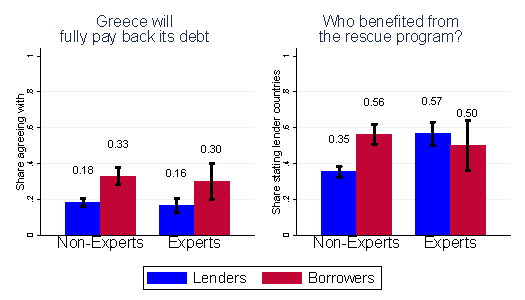
\includegraphics[scale=1.2]{graph6.pdf}

    \label{fig:figure10}
    \end{center}
    \tiny
    \begin{tablenotes}
     {The exact wording of the questions is: The two remaining questions are specifically about Greece. Question 6: Greece will fully pay back it's debt ; Answer options strongly agree, slightly agree, slightly disagree, strongly disagree, I don't know
    Question 7: Who primarily benefited from the loans granted to Greece; Answer options:  Greece, The lender countries, Both benefited equally, I don't know. We exclude all participants that answered the question with I don't know. \\
    The whiskers represent the 95 \% confidence intervals. }
    \end{tablenotes} 
\end{figure}


The results show that both non-experts and experts from borrower countries (0.33 and 0.30) believe to a larger extent than non-experts and experts from lender countries (0.18 and 0.16) that Greece will fully pay its debt; a result that indicates a nation-serving bias. The observed differences are statistically significant for the sample of non-experts and experts.  

 \clearpage
 The results also show that the fraction of non-experts from lender countries (0.35) is much smaller than the fraction of non-experts from borrower countries (0.56) believing that Greece benefited from the rescue program. Inferences based on the unconditional correlations in Figure 10 are corroborated by the conditional correlations reported in Figure 11.
 \\
\begin{figure}[h!] 
\begin{center}
     \caption{Situation in Greece}
     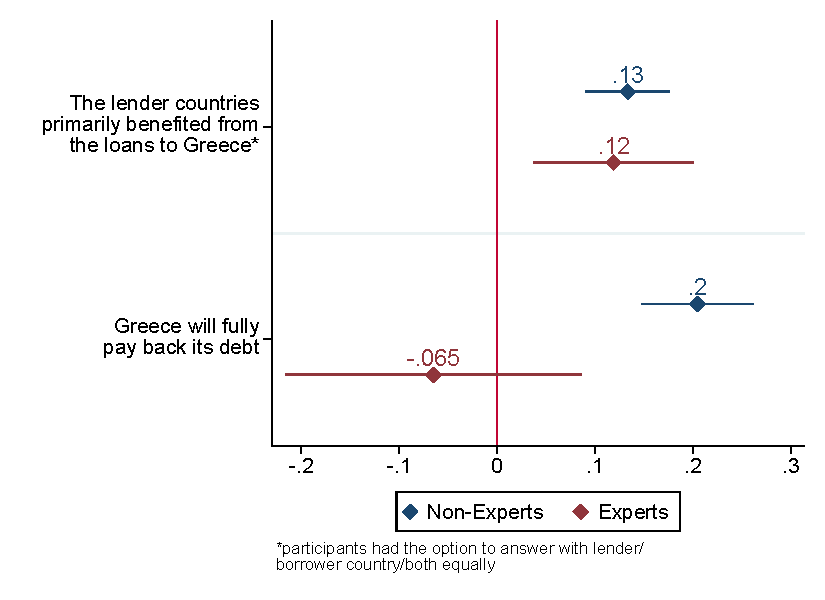
\includegraphics[scale=0.8]{Question6_7_base.pdf}
     \label{fig:my_label}
     \end{center}
     \tiny
     \tablenotes{The exact wording of the question is.   Question 6: Who primarily benefited from the loans to Greece; Question 7: Greece will fully pay back it's debt}
\end{figure}
\section{Robustness Checks}
\subsection{Robustness Checks (long) }
We estimate our model again on the subset of countries that share individual common characteristics with the lender countries. We examine the sample of countries which experienced a high level of unemployment growth, high level of debt growth and a low level of GDP growth during the years after the great recession and the European debt crisis namely from 2007 to 2012. We also consider the subset of countries which  were from the Southern part of the European Union \footnote{We employ the Wikipedia definition}, countries located more at the periphery \footnote{as measured by distance form Brussels} and part of the Eurozone. The baseline results remain unchanged among these sample splits.   When asked about the intentions behind entering the rescue program the findings from the baseline regression persist among all sample splits. The effect in the sample of countries with high levels of unemployment becomes smaller and is only significant at the five percent level. In the sample of southern European countries the disagreement over whether lender countries wanted to impose institutional change on borrower countries also decreases and is only significant at the five percent level. Interestingly, the estimates for the sample of periphery countries are much larger than in the baseline sample. In the periphery sample participants from program countries are 19.1 percentage points less likely to agree with the statement that the lender countries wanted to help the borrowing countries and 14.2 percentage points more likely to agree that lender countries wanted to impose institutional change compared to 13.1 and 11.1 percentage points in the full sample.\\
When asked about the emotions of citizens in borrower and lender countries the estimates become slightly smaller in the southern European, periphery and high debt sample than for the full sample. The divergence in assessments about whether the rescue program made the citizens in the borrower countries feel inferior even becomes insignificant in the Southern European sample. Among bot samples there is substantial disagreement between program and non-program countries that Greece will repay it's debt. 
\\
\begin{figure} [h!]
    \begin{center}
     \caption{ Intentions of the borrower countries}
    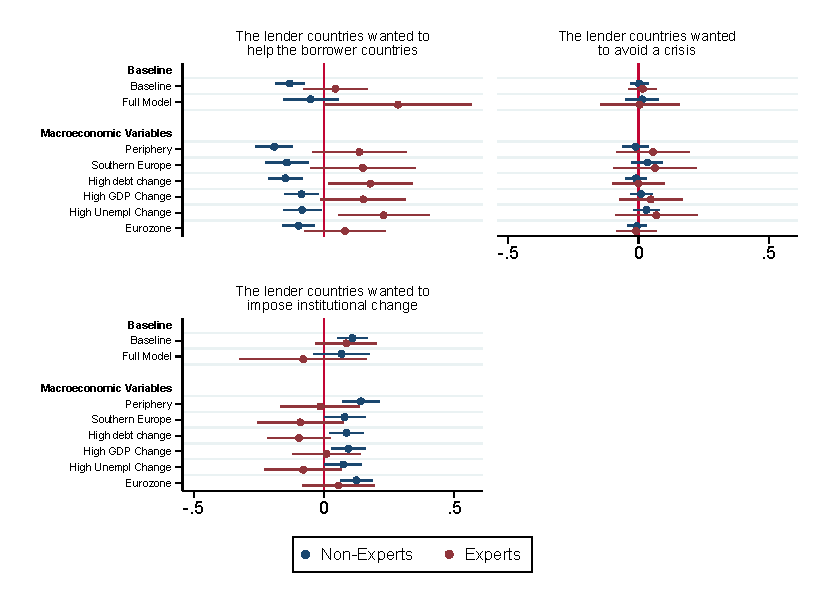
\includegraphics[scale=1.2]{Question2_samplesplits.pdf}
    \label{fig:my_label}
    \end{center}
    \tiny 
    \tablenotes{Participants were asked to assess the following statements:  Question 2.1: The lender countries wanted to help the borrowing countries Question 2.2: The lender countries wanted to help themselves avoid a crisis at home Question 2.3: The lender countries wanted to impose institutional change upon the borrower countries }
\end{figure}
\begin{figure}[h!]
    \begin{center}
     \caption{Sentiments of borrower countries (Macro Variables)}
    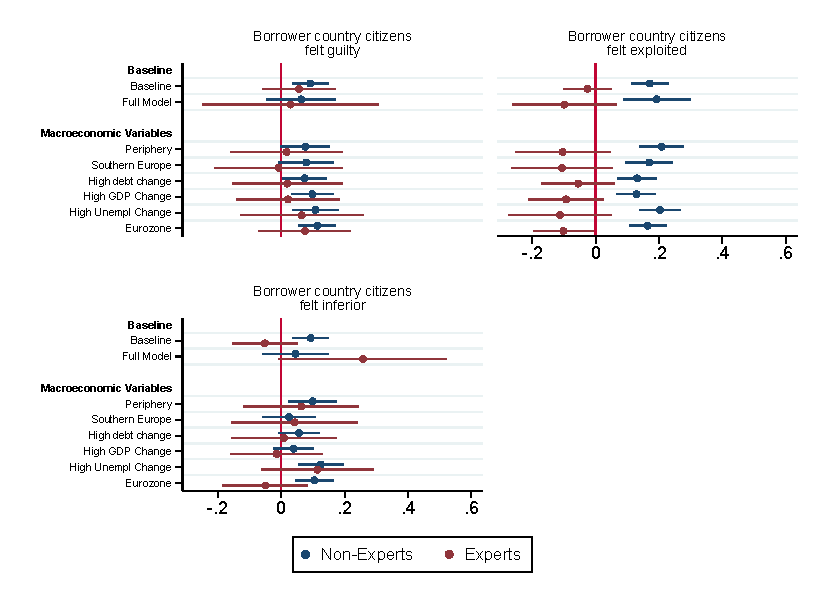
\includegraphics[scale=1.2]{Question51_samplesplits.pdf}
    \label{fig:my_label}
    \end{center}
    \tiny 
     \tablenotes{Question 5.1: The rescue experience made many citizens in the borrower countries feel guilty; Question 5.2: The rescue experience made many citizens in the borrower countries feel exploited; Question 5.3: The rescue experience made many citizens in the borrower countries feel inferior} 
\end{figure}
\begin{figure}[h!]
    \begin{center}
     \caption{Sentiments of lender countries(Macro Variables)}
    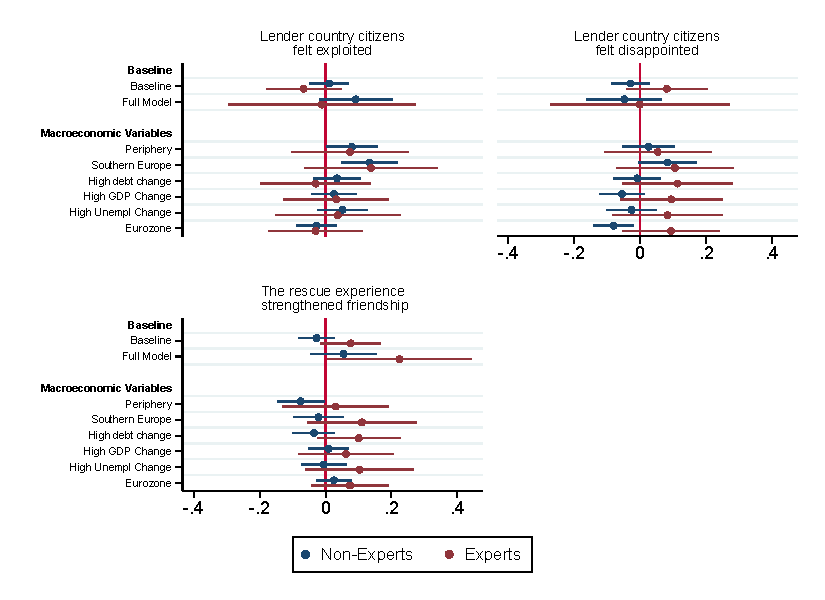
\includegraphics[scale=1.2]{Question52_samplesplits.pdf}
    \end{center}
    \tiny
     \tablenotes{Question 5.4: The rescue experience made many citizens in the lender countries feel exploited; Question 5.5 The rescue experience made many citizens in the lender countries feel disappointed Question 5.6: The rescue experience strengthened friendships between citizens Question 7: Greece will fully pay back it's debt}
\end{figure}
\begin{figure}[h!]
    \begin{center}
     \caption{Who initiated and benefited from the rescue program (Macro Variables)}
    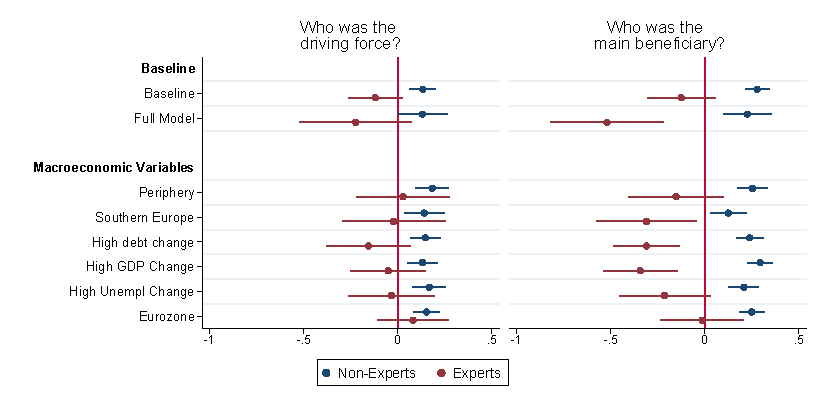
\includegraphics[scale=1.2]{macro_S_1301_S_1401.pdf}
    \end{center}
    \tiny
    \tablenotes{Question 3: Who was the driving force behind signing the memorandum; Question 4: Who was the main beneficiary of the program; }
\end{figure}
    
\begin{figure}[h!]
    \begin{center}
     \caption{Situation in Greece (Macro Variables}
    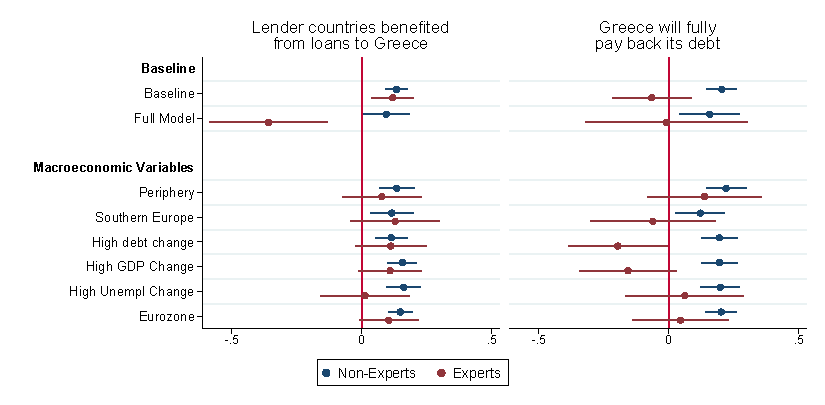
\includegraphics[scale=1.2]{macro_S_1601_S_1701.pdf}
    \end{center}
    \tiny
    \tablenotes{Question 6: Who primarily benefited from the loans to Greece; Question 7: Who primarily benefited from the loans to Greece}
\end{figure}
    \clearpage
\textbf{Ordered and Multinomial Estimation}
In the baseline model we aggregate the response options into two different categories, namely whether participants agree or do not agree with a statement.  To control if differences between participants from non-program and program countries also emerge when including all answer possibilities as regression outcomes we estimate multinomial and ordered logit models. For all questions in which participants were asked to rank their level of agreement we estimate an ordered logit model, for questions in which participants were asked to name the responsible party we estimate an multinomial logit model. The significance level in the non-expert sample remains at the same level for all but one question. For the question which party was the driving force behind the referendum the significance level changes from 0.01 percent to 0.05 percent. In the expert sample all results remain insignificant. For the question if Greece will repay it's debt the divergence in effects is only significant at the 5 percent level and no longer the 1 percent level. In the majority of cases the the magnitude of effects is the same for different answer possibilities. This suggests that differences between program and non-program countries exist across all answer possibilities. \\

\\
\textbf{Inattentive Respondents}
Since we distributed our survey for the non-expert sample online we will also control for the influence of inattentive respondents in the non-expert sample. When distributing the survey online we already included an attention check when asking participants about socioeconomic characteristics. All participants failing this attention check were excluded from the survey. Further, we exclude all participants at the top 10 $\%$ and bottom 10 $\%$ of the survey time distribution. Excluding these participants does not change the inferences of our baseline estimation in the non-expert sample.\\


\\
\textbf{Clustered Robust Standard Errors} 
We cluster standard errors on the country level. Due to the limited number of member states of the European Union we adjust for the small number of clusters using the wild bootstrap method for logit regressions as suggested by \cite{cameron}.\footnote{We use the Stata command developed by \cite{roodman}} Inferences change for some questions when applying this method. Question 2.c becomes insignificant, questions 5a and 5c loose some significance and become significant at the 5 respectively 10 percent level.  \\

\textbf{Multiple Hypothesis Testing}
We also control for multiple hypothesis testing by adjusting our p-values using the Bonferroni Method. We adjust p-values by the number of questions we ask our participants. The Bonferroni correction does not change the significance level of our results. 

%\subsection{Robustness Checks short} 
%Borrower and lender countries vary along other dimensions than the borrower/ lender distinction. Program countries share several characteristics which are likely to influence the estimates. Countries which were affected by the European debt crisis are predominantly Southern European and are located at the periphery of the European Union (measured by distance to Brussels). Further, all these countries experienced a substantial increase in debt levels, high levels of unemployment, low GDP growth and belonged to the Eurozone. Thus we conduct sample splits along these margins to test whether these variables drive our results. \footnote{ We again estimate our model on the subsample of countries which are Southern European, belong to the Eurozone,are located at the periphery of Europe,defined as countries in which the distance of the capital to Brussels is above the median, experienced above median debt and unemployment growth and below median GDP growth during the years 2007 and 2012.} The overall findings of our analysis remain unchanged among the expert and non-expert sample.
%\\
%In addition to controlling for the influence of macroeconomic variables we also conduct several other robustness checks. We estimate the model by ordered and multinomial estimation, we cluster standard errors at the country level, control for multiple hypothesis testing and drop inattentive respondents from our non-expert sample. All these checks do not yield substantially different results than our baseline estimation. A detailed overview of the results of our heterogeneity analysis and robustness checks can be found in the appendix. 

\section{Conclusion} 
The 2010 European public debt crisis influenced policies, politics and voters' perceptions. For example, domestic policy-makers introduced measures such as fiscal rules to handle increasing public debt and budget deficits. The European Central Bank pursued expansionary monetary policies: it introduced the Outright Monetary Transactions (OMT) program and decreased interest rates to zero. Rescue programs for Cyprus, Greece, Ireland, Portugal and Spain were designed. 

We examined citizens' views about the European public debt crisis. In particular, we investigated collective memory of the European public debt crisis and disentangled views of citizens from borrower countries and citizens from lender countries. During the public debt crisis, media reports have suggested that citizens from borrower and lender countries have different views on the crisis and how to handle it. Studies in psychology suggest that individual borrowers and lenders remember credit relationships in different manners (\cite{dezso}): memories are influenced by a self-serving bias. It is conceivable that such self-serving bias gives rise to a nation-serving bias in the memory of national credit relationships. We examine a nation-serving bias in memories of national credit relationships. Doing so is new.

We compiled new data measuring collective memories on the European debt crisis. We asked economic experts by using CESifo's World Economic Survey and non-experts by using the provider prolific. The results suggest that experts from lender and borrower countries have quite similar views about the European public debt crisis. The views of non-experts are, by contrast, influenced by a nation-serving bias. The bias relates to memories on why countries signed a memorandum and how they assess the measures taken to address the crisis. These results corroborate empirical studies about citizens' misperceptions about macroeconomic policies and outcomes. Citizens evaluate macroeconomic policies and outcomes much better when their preferred political party is in office than when parties govern that they do not support (on partisan bias see, for example, \cite{evans}, \cite{gerber}, \cite{gillitzer}, \cite{bachmann}). 

We observe a much smaller nations-serving bias among non-experts when we examine non-experts that left their country of birth. Cosmopolitans are less likely to evaluate European policies with a nation-serving bias than non-Cosmopolitans (see also \cite{bechtel}).

We believe that citizens' misperceptions and nation-serving bias in memorizing and handling European events are a major issue for European countries. When citizens have misperceptions and nation-serving bias in memorizing and handling European events, citizens are likely to demand policies that they would not demand when being suitably informed. Platforms of established political parties converged in many European countries. Established political parties did not wish to offer polarized in dealing with the public debt crisis. Many citizens were disenchanted and, in turn, new populist political parties entered the political arena. Clearly, citizens' views about the public debt crisis and their perceptions about European policies gave rise to electoral success of new (populist) parties and, in turn, reinforced policies in Europe. 

Our study shows divergences in how European policies between European countries are perceived. Moreover, experts who advise politicians do not tend to have misperceptions about the European public debt crisis. Misperceptions among non-experts but no misperceptions among experts and policy-makers may well explain why European policies and the EU as an institution is considered as unpopular in many countries. 

We believe that (social) media influence citizens' views a great deal. An avenue for future research is examining the extent to which social media influence misperceptions and nation-serving bias. 
\clearpage
\section{Appendix}
\subsection{Sample Splits: Suggestion 1}
\begin{figure} [h!]
    \begin{center}
     \caption{Hypothesis 1: Intentions of the borrower countries}
    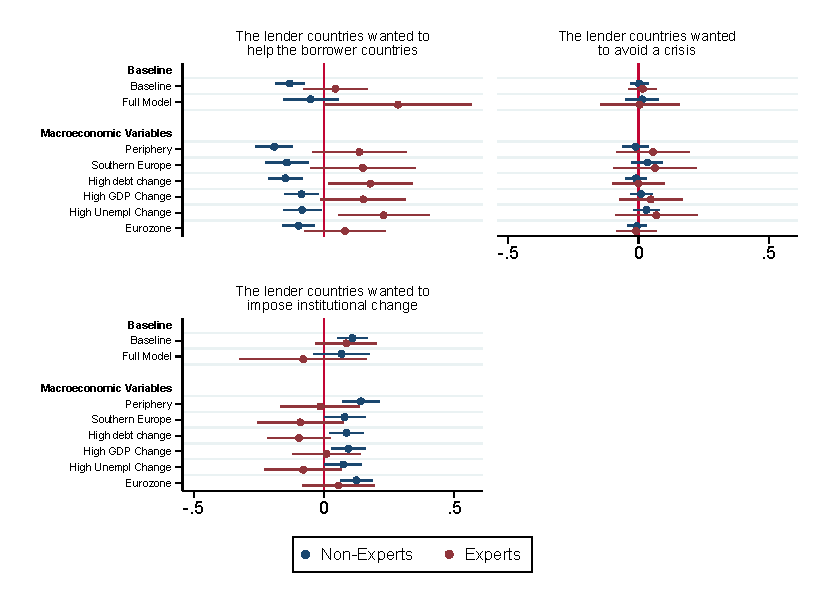
\includegraphics[scale=1.2]{Question2_samplesplits.pdf}
    \label{fig:my_label}
    \end{center}
    \tiny 
    \tablenotes{Participants were asked to assess the following statements:  Question 2.1: The lender countries wanted to help the borrowing countries Question 2.2: The lender countries wanted to help themselves avoid a crisis at home Question 2.3: The lender countries wanted to impose institutional change upon the borrower countries }
\end{figure}
\begin{figure}[h!]
    \begin{center}
     \caption{Hypothesis 4: Emotions of program countries}
    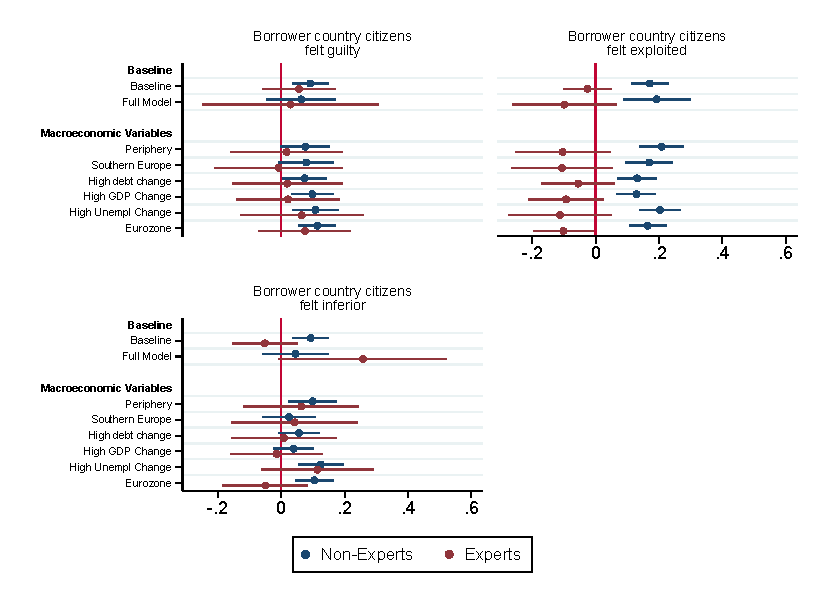
\includegraphics[scale=1.2]{Question51_samplesplits.pdf}
    \label{fig:my_label}
    \end{center}
    \tiny 
     \tablenotes{Question 5.1: The rescue experience made many citizens in the borrower countries feel guilty; Question 5.2: The rescue experience made many citizens in the borrower countries feel exploited; Question 5.3: The rescue experience made many citizens in the borrower countries feel inferior} 
\end{figure}
\begin{figure}[h!]
    \begin{center}
     \caption{Hypothesis 4: Emotions of non-program countries and repayment of outstanding debt}
    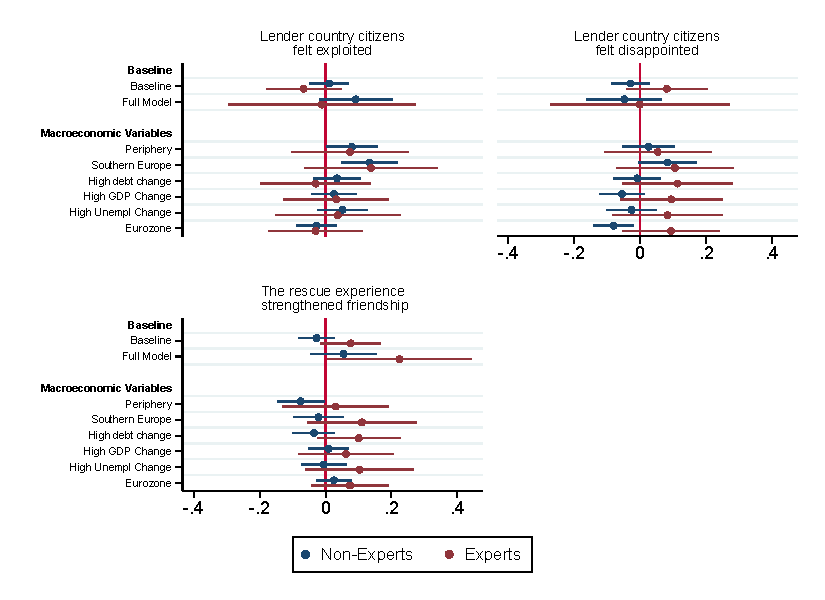
\includegraphics[scale=1.2]{Question52_samplesplits.pdf}
    \end{center}
    \tiny
     \tablenotes{Question 5.4: The rescue experience made many citizens in the lender countries feel exploited; Question 5.5 The rescue experience made many citizens in the lender countries feel disappointed Question 5.6: The rescue experience strengthened friendships between citizens Question 7: Greece will fully pay back it's debt}
\end{figure}
\begin{figure}[h!]
    \begin{center}
     \caption{Hypothesis 2 and 3: Who initiated and benefited from the rescue program}
    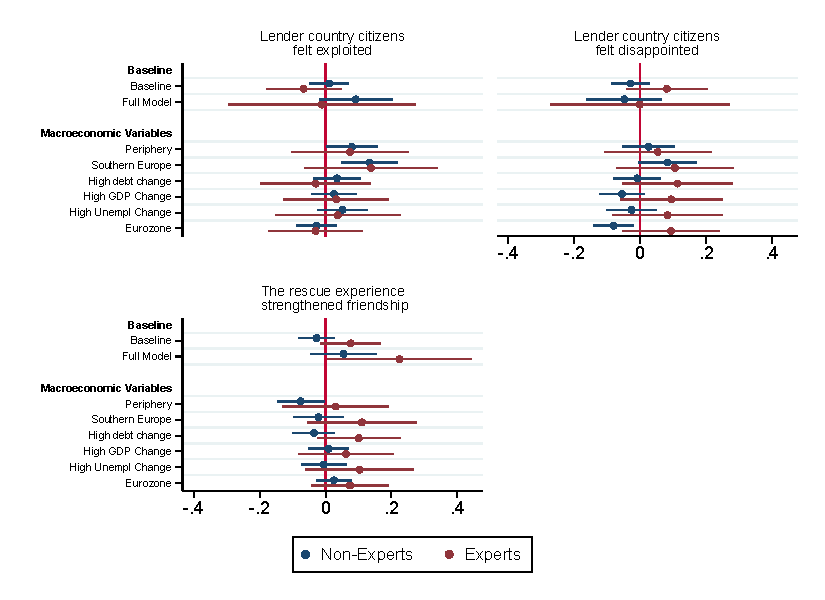
\includegraphics[scale=1.2]{Question52_samplesplits.pdf}
    \end{center}
    \tiny
    \tablenotes{Question 3: Who was the driving force behind signing the memorandum; Question 4: Who was the main beneficiary of the program; Question 7: Who primarily benefited from the loans to Greece}
\end{figure}


\begin{figure}[h!]
\caption{Hypothesis 1: Intentions of the lender countries}
    \begin{minipage}{0.5\textwidth}

    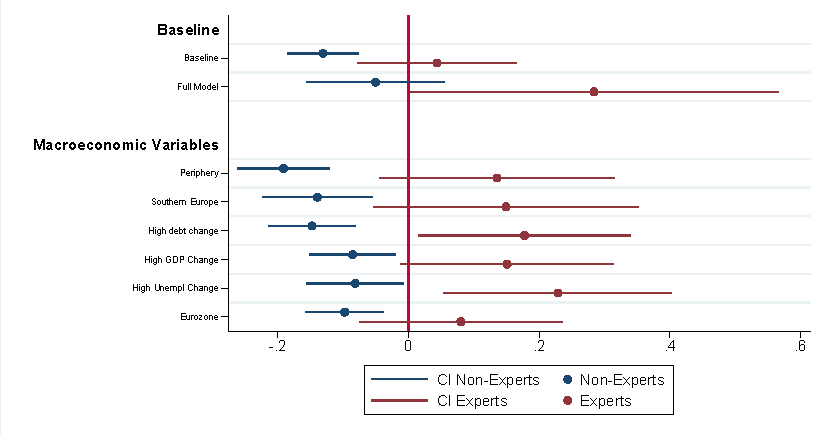
\includegraphics[scale=0.65]{QuestionS_1201.pdf}
    \footnotesize{
     \subcaption{Question 2.1}}
\end{minipage}
\begin{minipage}{0.5\textwidth}
    
    
    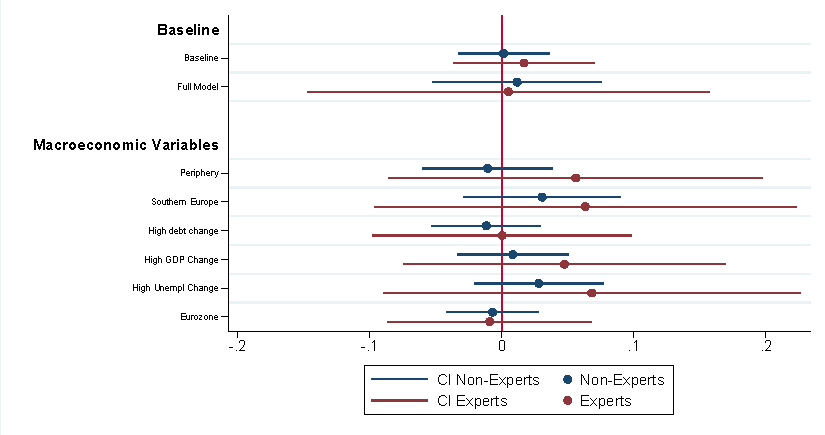
\includegraphics[scale=0.65]{QuestionS_1202.pdf}
        \footnotesize{
        \subcaption{Question 2.2} }
\end{minipage} 
 \begin{minipage}{0.5\textwidth}
  
    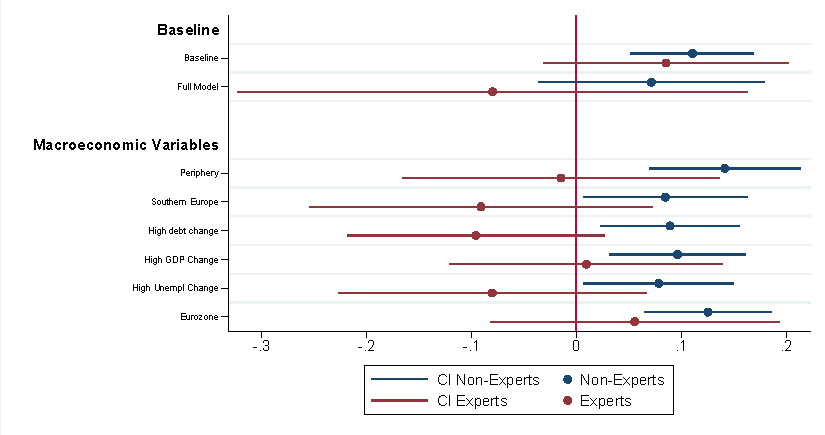
\includegraphics[scale=0.65]{QuestionS_1203.pdf}
    \footnotesize{
     \subcaption{Question 2.3}}
    \label{fig:my_label}
    \end{minipage}
     \begin{minipage}{0.5\textwidth}
         \end{minipage}
         \vskip 0.3cm
             \tiny 
    \tablenotes{Participants were asked to assess the following statements:  Question 2.1: The lender countries wanted to help the borrowing countries;  Question 2.2: The lender countries wanted to help themselves avoid a crisis at home; Question 2.3: The lender countries wanted to impose institutional change upon the borrower countries }

\end{figure} 



\begin{figure}[h!]
\caption{Hypothesis 4: Emotions evoked among citizens }
    \begin{minipage}{0.5\textwidth}
    
    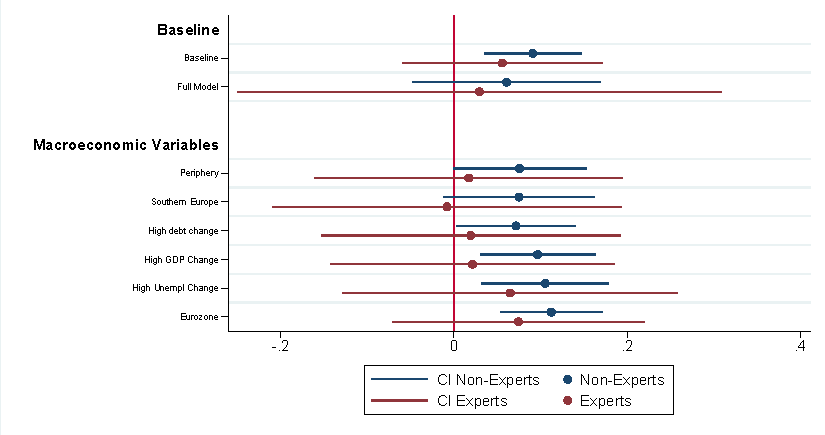
\includegraphics[scale=0.65]{QuestionS_1501.pdf}
    \footnotesize{
     \subcaption{Question 5.1} }
\end{minipage}
\begin{minipage}{0.5\textwidth}
    \centering
    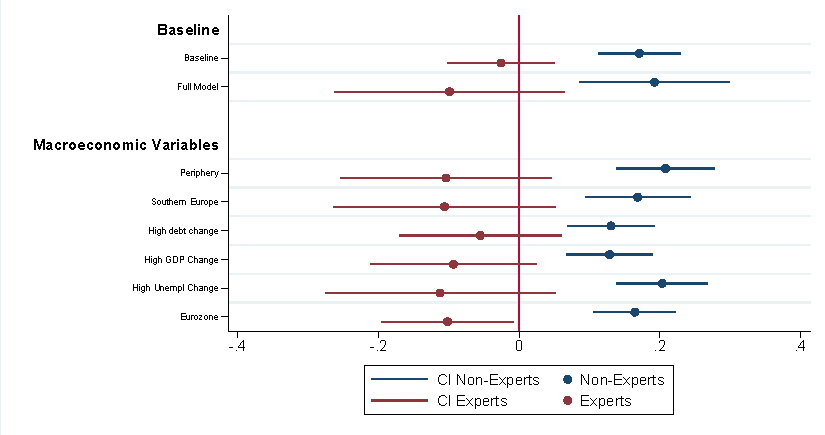
\includegraphics[scale=0.65]{QuestionS_1502.pdf}
    \footnotesize{
      \subcaption{Question 5.2}}
\end{minipage} 
 \begin{minipage}{0.5\textwidth}
    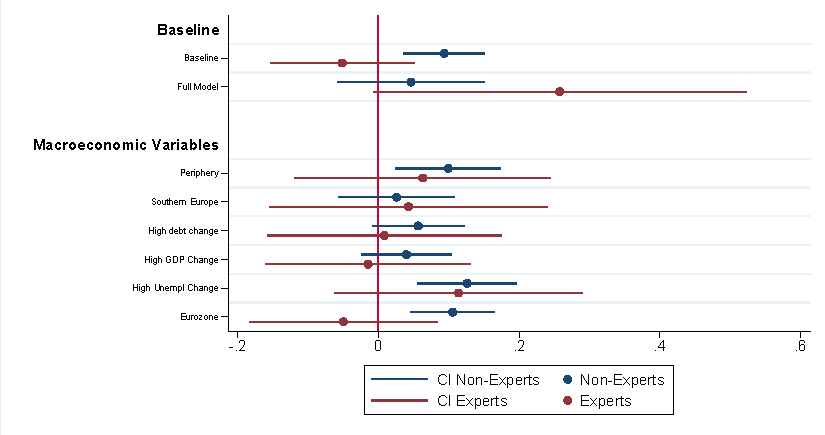
\includegraphics[scale=0.65]{QuestionS_1503.pdf}
    \footnotesize{
     \subcaption{Question 5.3}}
    \label{fig:my_label}
    \end{minipage}
     \begin{minipage}{0.5\textwidth}
    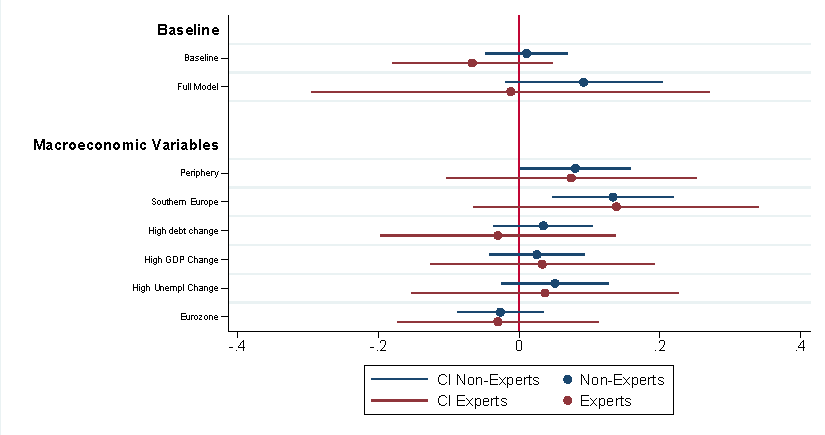
\includegraphics[scale=0.65]{QuestionS_1504.pdf}
    \footnotesize{
     \subcaption{Question 5.4}}
    \label{fig:my_label}
    \end{minipage}
     \begin{minipage}{0.5\textwidth}
    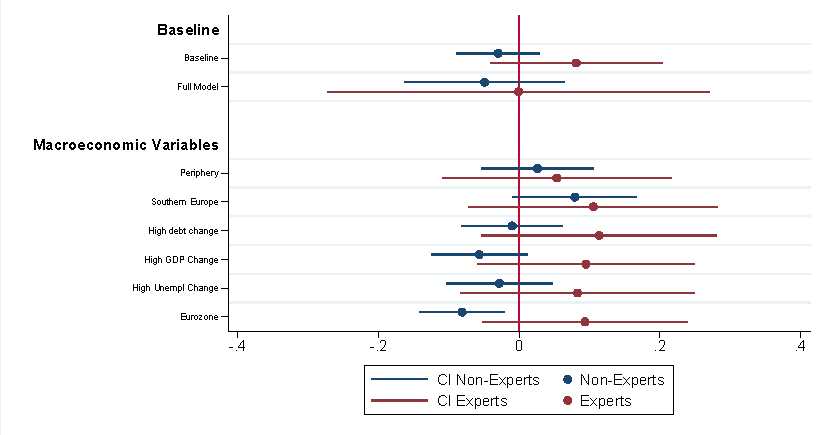
\includegraphics[scale=0.65]{QuestionS_1505.pdf}
    \footnotesize{
     \subcaption{Question 5.5}}
    \label{fig:my_label}
    \end{minipage}
     \begin{minipage}{0.5\textwidth}
    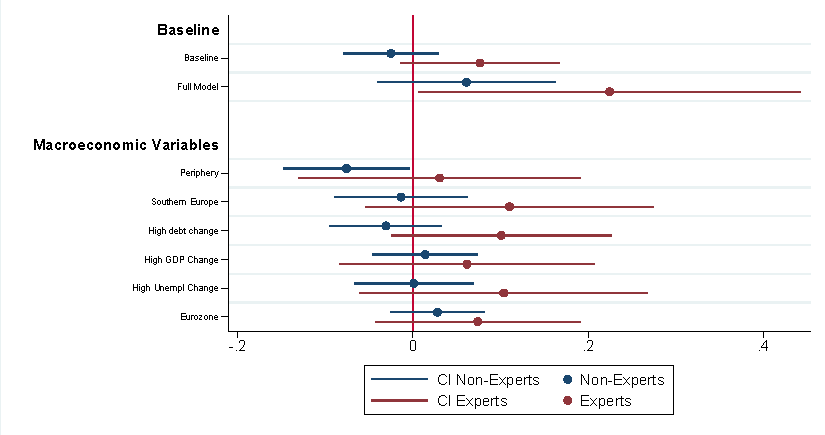
\includegraphics[scale=0.65]{QuestionS_1506.pdf}
    \footnotesize{
     \subcaption{Question 5.6}}
    \label{fig:my_label}
    \end{minipage}
    \vskip 0.3cm
        \tiny
     \tablenotes{Question 5.1: The rescue experience made many citizens in the borrower countries feel guilty; Question 5.2: The rescue experience made many citizens in the borrower countries feel exploited; Question 5.3: The rescue experience made many citizens in the borrower countries feel inferior; Question 5.4: The rescue experience made many citizens in the lender countries feel exploited; Question 5.5 The rescue experience made many citizens in the lender countries feel disappointed; Question 5.6: The rescue experience strengthened friendships between citizens; Question 7: Greece will fully pay back it's debt}
\end{figure} 

\begin{figure}[h!]
\caption{Driving force and beneficiaries of the program}
    \begin{minipage}{0.5\textwidth}
    
    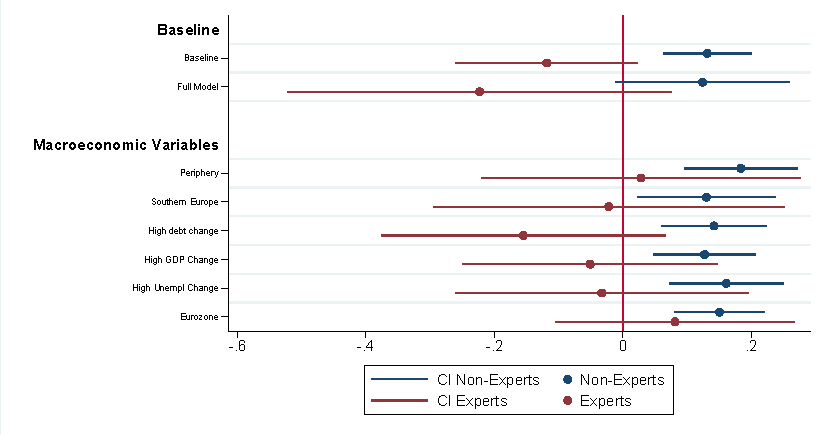
\includegraphics[scale=0.65]{QuestionS_1301.pdf}
    \footnotesize{
     \subcaption{Question 3} }
\end{minipage}
\begin{minipage}{0.5\textwidth}
    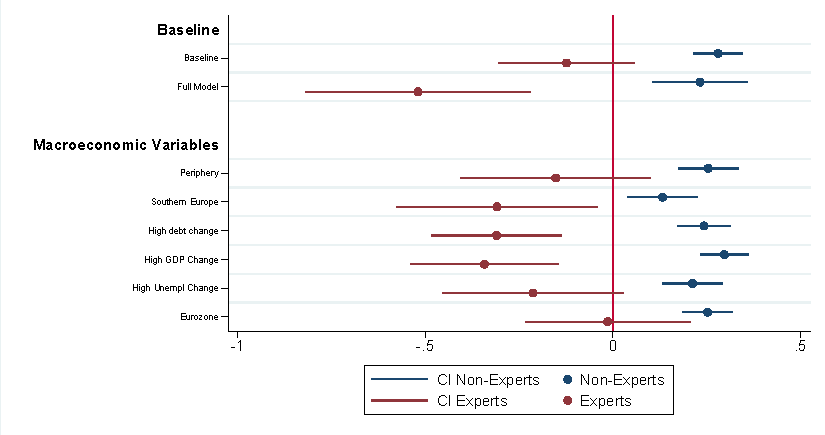
\includegraphics[scale=0.65]{QuestionS_1401.pdf}
    \footnotesize{
      \subcaption{Question 4}
      }
\end{minipage} 
 \begin{minipage}{0.5\textwidth}
  
    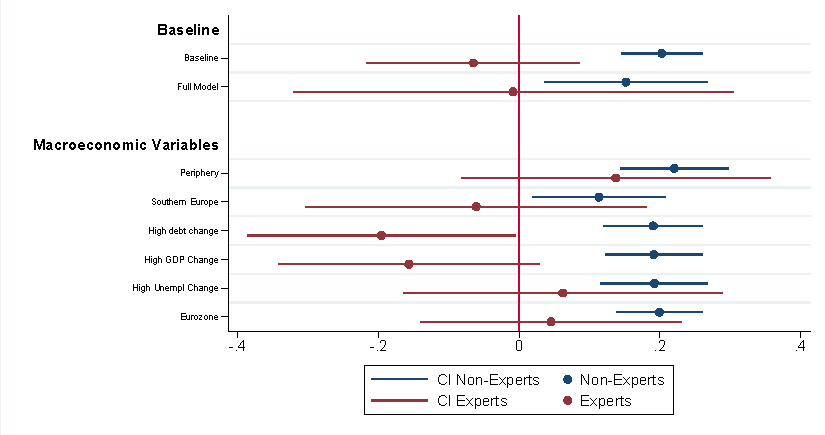
\includegraphics[scale=0.65]{QuestionS_1701.pdf}
    \footnotesize{
     \subcaption{Question 7}}
    \label{fig:my_label}
    \end{minipage}
    \vskip 0.3cm
        \tiny
    \tablenotes{Question 3: Who was the driving force behind signing the memorandum; Question 4: Who was the main beneficiary of the program; Question 7: Who primarily benefited from the loans to Greece}
\end{figure} 














\clearpage
\bibliographystyle{apalike}
\bibliography{bibliography.bib}
\end{document}
